\documentclass[letterpaper, 11pt]{article}
\usepackage{comment} % enables the use of multi-line comments (\ifx \fi) 
\usepackage{fullpage} % changes the margin
\usepackage{fancyhdr} % for footerhttps://www.overleaf.com/3039851kkndbp#
\usepackage[UKenglish]{isodate}% http://ctan.org/pkg/isodate for date format
\usepackage{float}%force tables/figs into certain placement
\usepackage{changepage}%for dichotomous key
\usepackage{graphicx}%for figures
\usepackage{caption}%for figures
\usepackage{subcaption}%for figures
\usepackage{hyperref}
\usepackage{textcomp}
\usepackage{natbib}
\usepackage{placeins}%prevent images from floating into inappropriate sections

\def\labelitemi{--}

\pagestyle{fancy}
\renewcommand{\headrulewidth}{0pt}

\lhead{}
\chead{}
\rhead{}
\lfoot{ENT 432 (Fall 2016) - Penn State}
\cfoot{}
\rfoot{\thepage}
\renewcommand{\footrulewidth}{0.4pt}
\title{Unit 6 - Non-pterygote Hexapoda}
\author{Open Entomology Project}

\begin{document}
\cleanlookdateon %removed ordinal date
\maketitle
\thispagestyle{fancy}
\section*{Introduction}
Here we begin looking at taxa classified in \textbf{Hexapoda}. In most cases you will examine multiple families, most of which you will be tested on in lab practicals. You may be shown more families than are on the handout---primarily so that you can better grasp the diversity that exists---but you will not have to sight-identify these other families. Looking at these other families may help to you, though, in identifying specimens for your collection. Some characters (in \textit{italics}) might be impossible to see but are provided for future reference.

\section*{Materials}

\begin{itemize}
\item specimens (provided)
\item fine forceps, probes (provided)
\item sorting tray, watch glasses, gloves, safety glasses, glycerine, ethanol (provided)
\item pencil/paper for sketches
\end{itemize}

\section*{Safety}
We will be working with sharp tools. Wear your personal protective gear at all times. Specimens are to be returned to their vials after lab, and glycerine and ethanol will be collected for proper disposal or reuse.

\section*{Methods}
Working with a partner, organize your space, specimens, tools, and microscope. Use your probe and forceps to manipulate the specimen. In this lab, however, we will not be dissecting specimens (unless otherwise noted). You can start anywhere in the handout.

\section*{Hexapoda}

\begin{itemize}
\item 3 tagmata: head, thorax, abdomen
\item 3 pairs of uniramous thoracic appendages (legs)
\end{itemize}

\subsection*{Entognatha}

\begin{itemize}
\item antennae, when present, truly segmented (\textit{i.e.}, each segment has intrinsic musculature)
\item tarsus not subdivided into tarsomeres (Figure \ref{fig:prottars})
\end{itemize}
Looking at the Figure \ref{fig:prothead} below, can you annotate the mouthparts of an entognathous hexapod? Mouthparts include the mandible but also the maxilla and the labium. Are these components all evaginated and visible?

\begin{figure}[ht!]
    \centering
    \begin{subfigure}[ht!]{0.45\textwidth}
        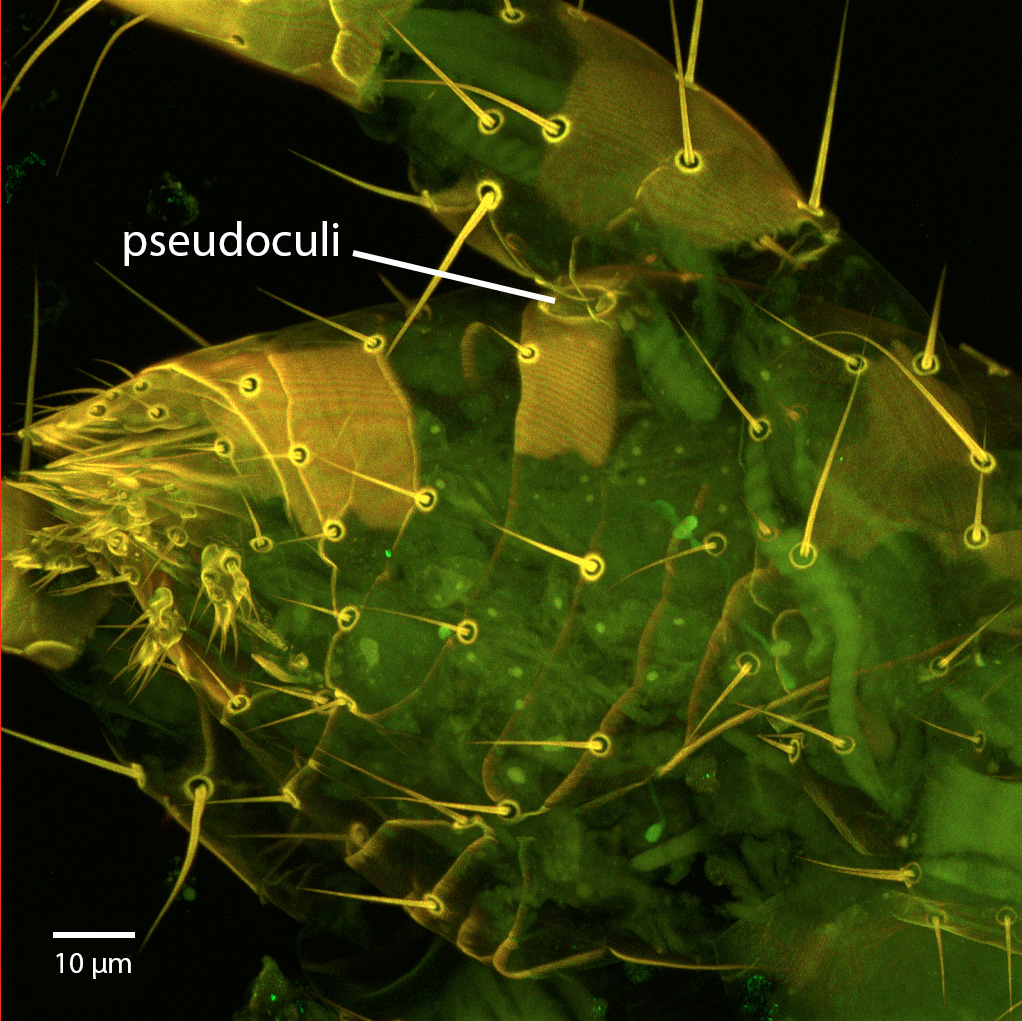
\includegraphics[width=\textwidth]{image21}
        \caption{CLSM volume rendered image showing proturan head (mouth region on the left-middle portion of the image) and base of fore leg. Photo (CC BY 2.0) by Istv\'an Mik\'o }
        \label{fig:prothead}
    \end{subfigure}
    ~ %add desired spacing between images, e. g. ~, \quad, \qquad, \hfill etc. 
      %(or a blank line to force the subfigure onto a new line)
    \begin{subfigure}[ht!]{0.45\textwidth}
        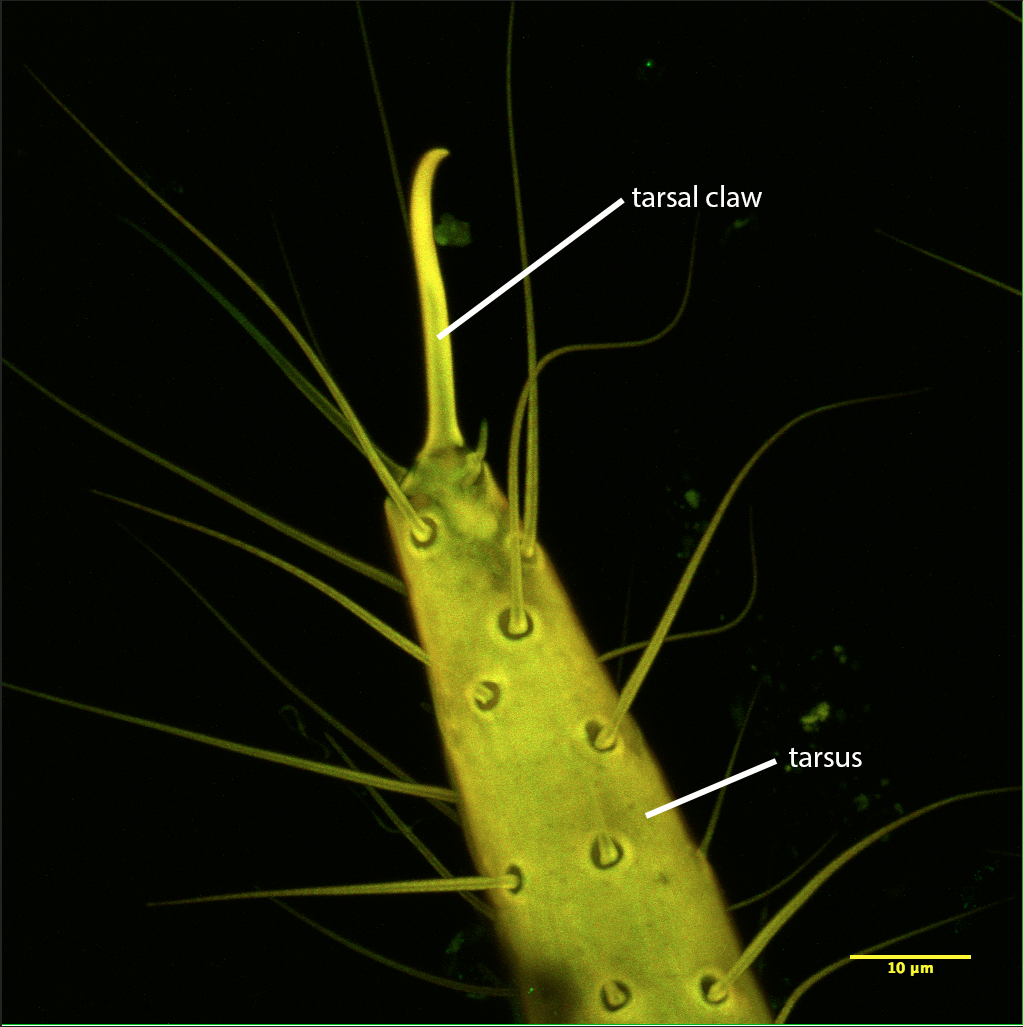
\includegraphics[width=\textwidth]{image23}
        \caption{CLSM volume rendered image showing proturan fore tarsus. Photo  (CC BY 2.0) by Istv\'an Mik\'o}
        \label{fig:prottars}
    \end{subfigure}
    \caption{Protura}\label{fig:proturans}
\end{figure}

\section{Protura (coneheads)}
\begin{itemize}
\item antennae apparently absent (Figures \ref{fig:proturanhab}, \ref{fig:prothead1})
\item eyes absent; \textit{sensory organs (pseudoculi) present where one would expect eyes to be}
\item \textit{mandibles without molar area (proximal flattened region for grinding food)}
\item body very small (\textless1.5 mm long)
\item abdomen 11-segmented, cerci absent (Figure \ref{fig:protapex})
\end{itemize}

\noindent{}How might the absence of antennae be adaptive for these hexapods? Where would you predict they live? Which structure functions as the primary anterior sensory appendage? \vspace{4cm} 

\begin{figure}[ht!]
  \centering
    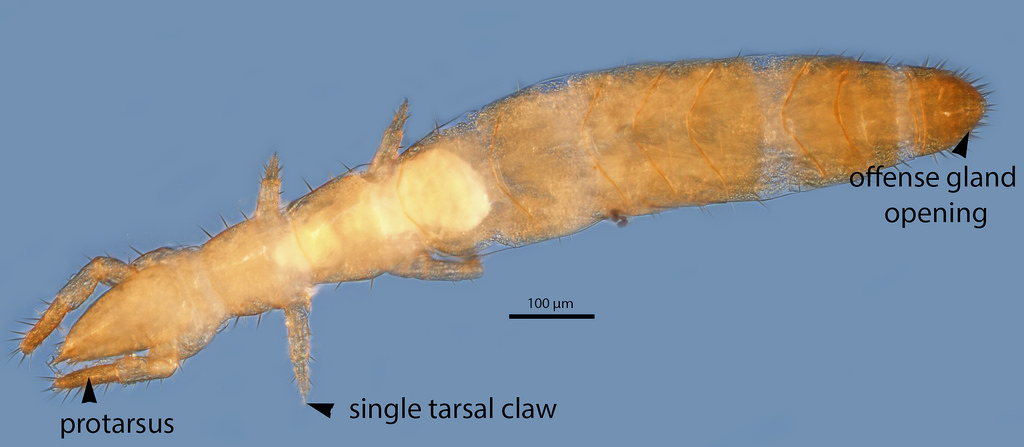
\includegraphics[width=0.8\textwidth]{protVent}
  \caption{Proturan habitus. Photo (CC BY 2.0) by Istv\'an Mik\'o \url{https://flic.kr/p/yCpxwp}}
  \label{fig:proturanhab}
\end{figure}

\begin{figure}[ht!]
    \centering
    \begin{subfigure}[ht!]{0.33\textwidth}
        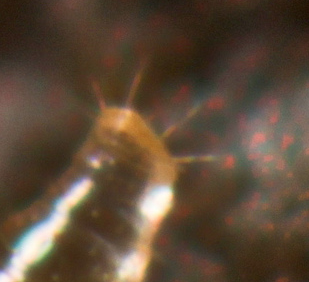
\includegraphics[width=\textwidth]{image06}
        \caption{Apex of abdomen. Photo (CC BY-SA 2.0) by Andy Murray \url{https://flic.kr/p/eaKZ2B}}
        \label{fig:protapex}
    \end{subfigure}
    ~ %add desired spacing between images, e. g. ~, \quad, \qquad, \hfill etc. 
      %(or a blank line to force the subfigure onto a new line)
    \begin{subfigure}[ht!]{0.35\textwidth}
        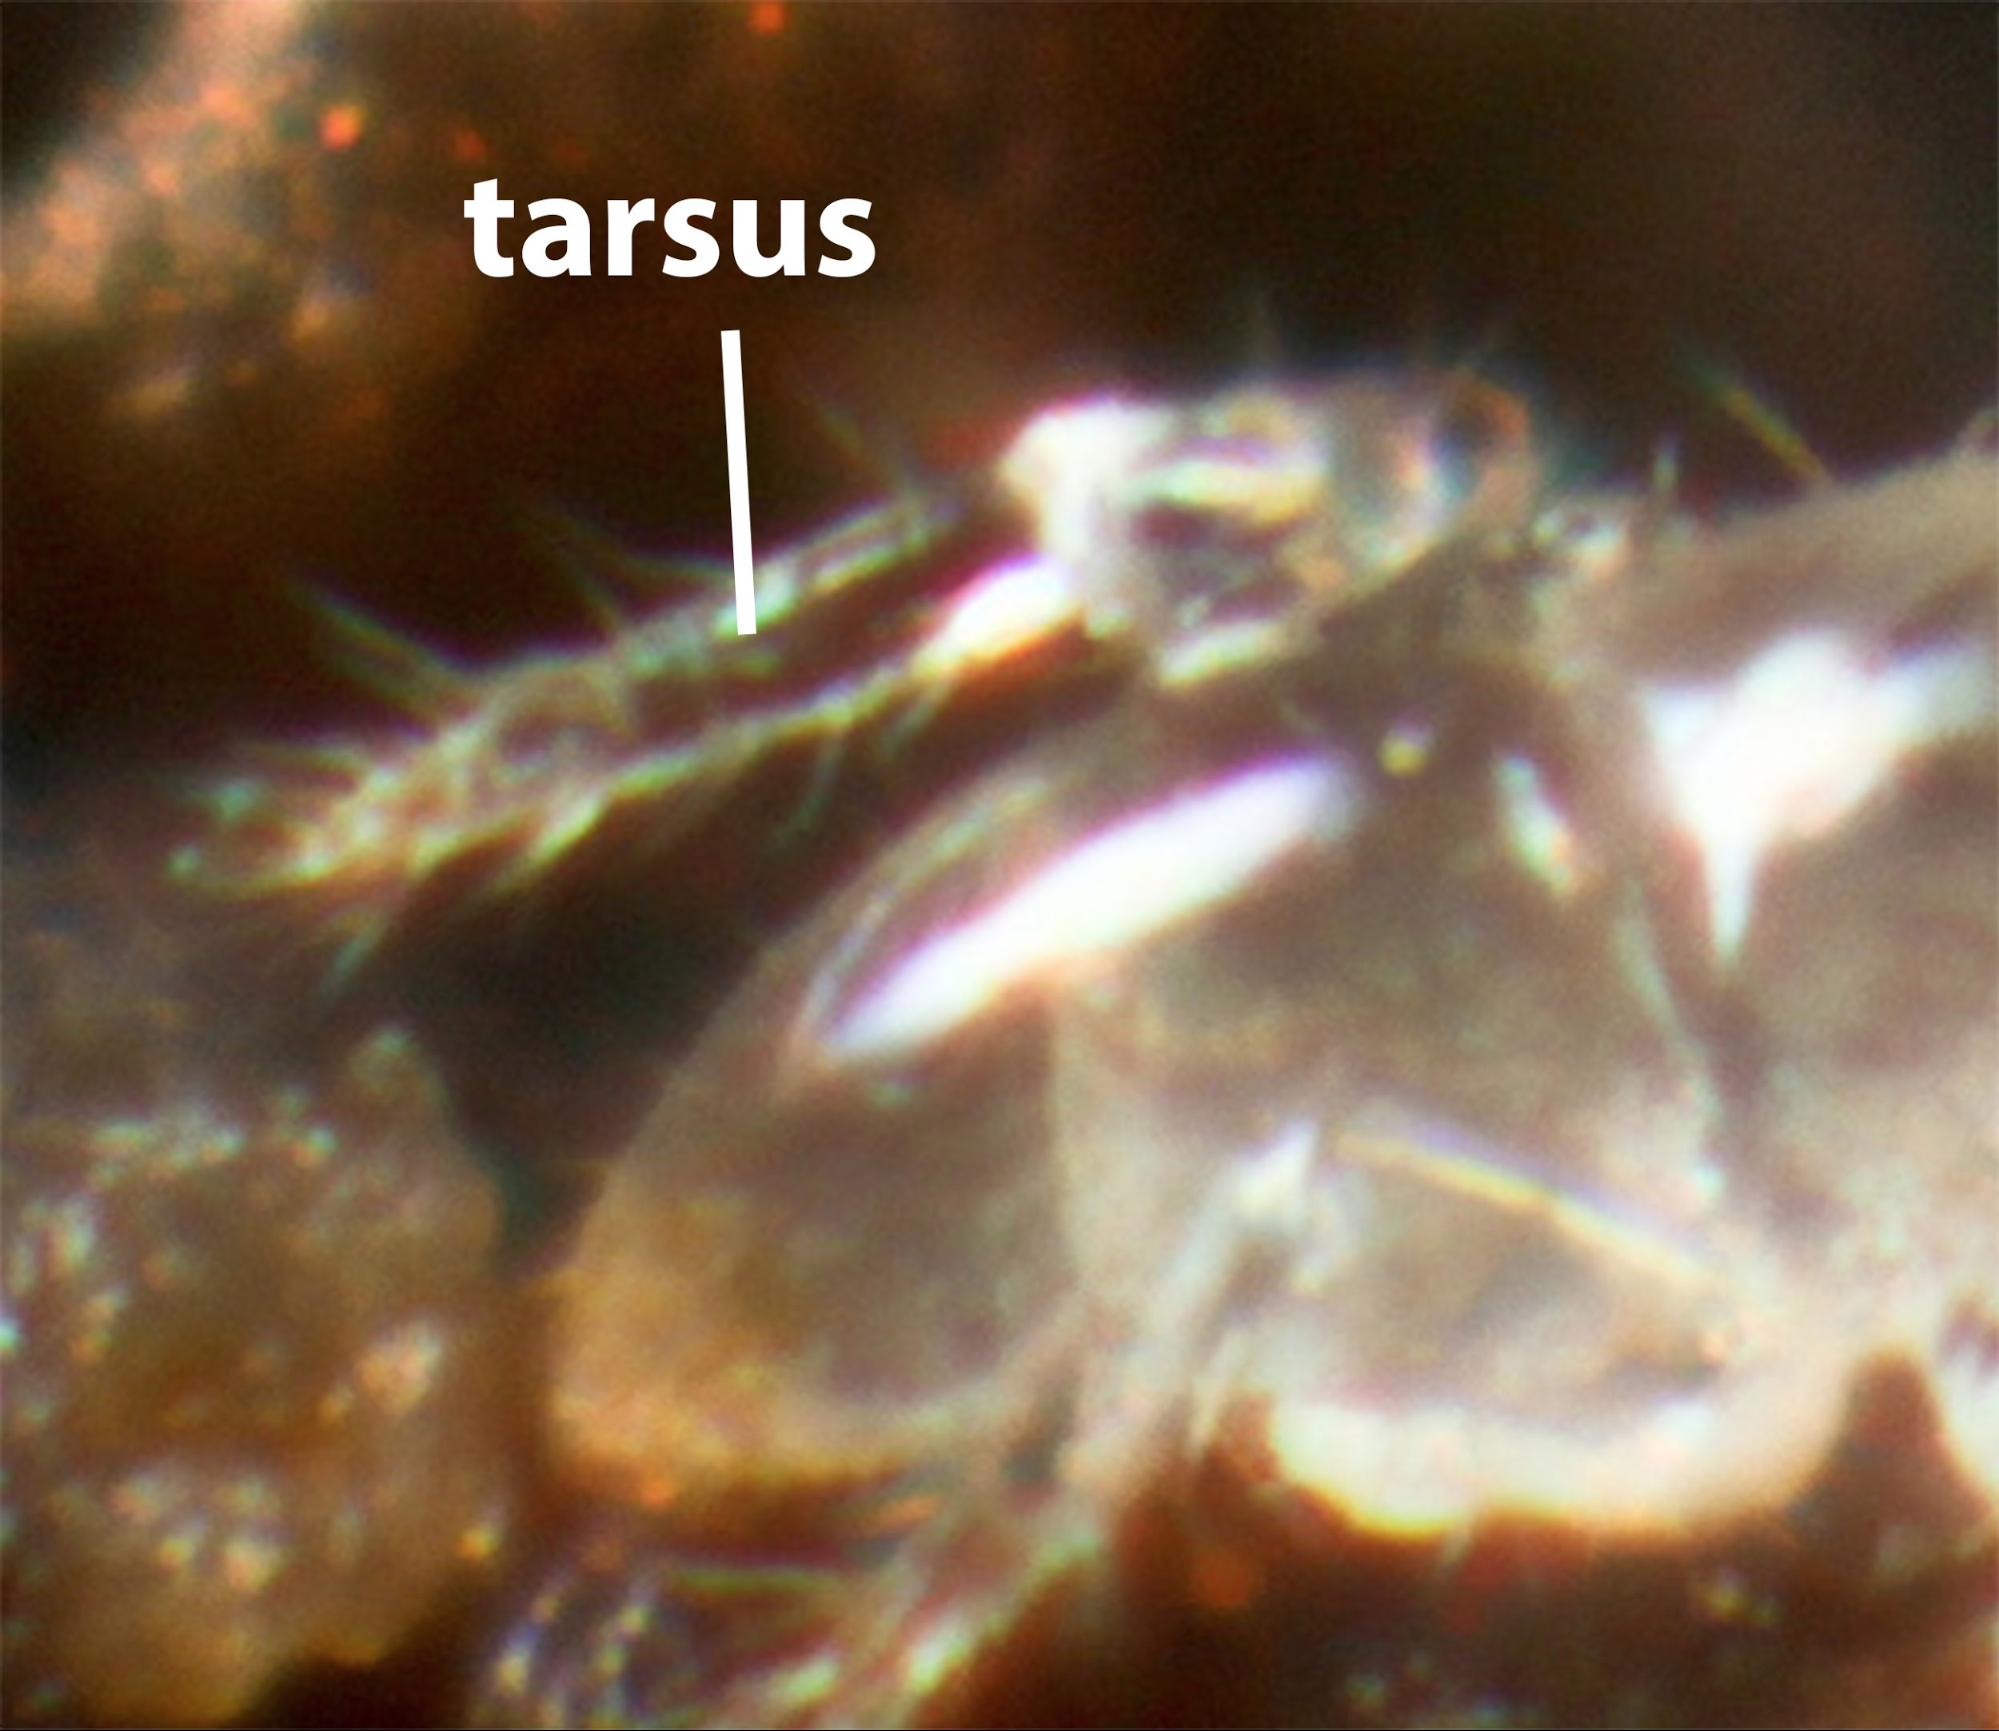
\includegraphics[width=\textwidth]{image30}
        \caption{Head and prothorax. Photo (CC BY-SA 2.0) by Andy Murray \url{https://flic.kr/p/eaKZ2B}}
        \label{fig:prothead1}
    \end{subfigure}
    \caption{Protura}\label{fig:proturanmorph}
\end{figure}

\section{Diplura (diplurans)}
\begin{itemize}
\item antennae filiform
\item eyes absent; pseudoculi absent 
\item \textit{mandibles without molar area}
\item body usually \textgreater3 mm long
\item cerci distinct
\item \textit{abdominal segments often with styli}
\end{itemize}

\noindent{}Compare dipluran fore legs to those of proturans; notice any difference? Now, focusing on Diplura, compare \textbf{Japygidae} (Figure \ref{fig:japygidhab}) with \textbf{Campodeidae} (Figure \ref{fig:campodeidhab}). What is your hypothesis for why the cerci vary phenotypically between families? What is their function?\vspace{3cm}

\begin{figure}[ht!]
  \centering
    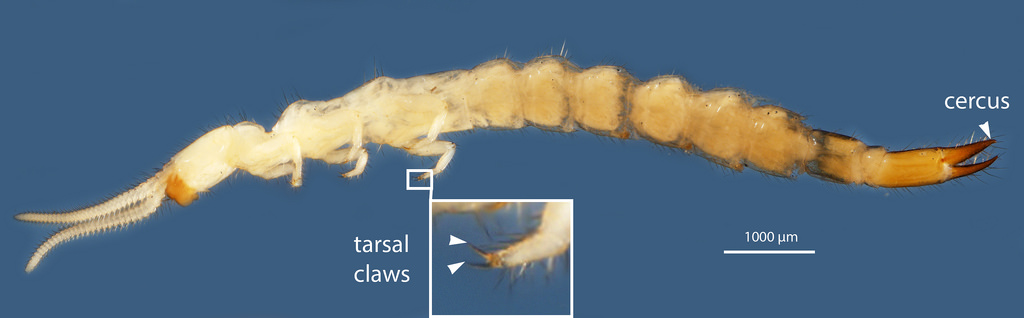
\includegraphics[width=0.9\textwidth]{japygid1}
  \caption{Japygidae habitus. Photo (CC BY 2.0) by Istv\'an Mik\'o  \url{https://flic.kr/p/yCo5BK}}
  \label{fig:japygidhab}
\end{figure}

\begin{figure}[ht!]
  \centering
    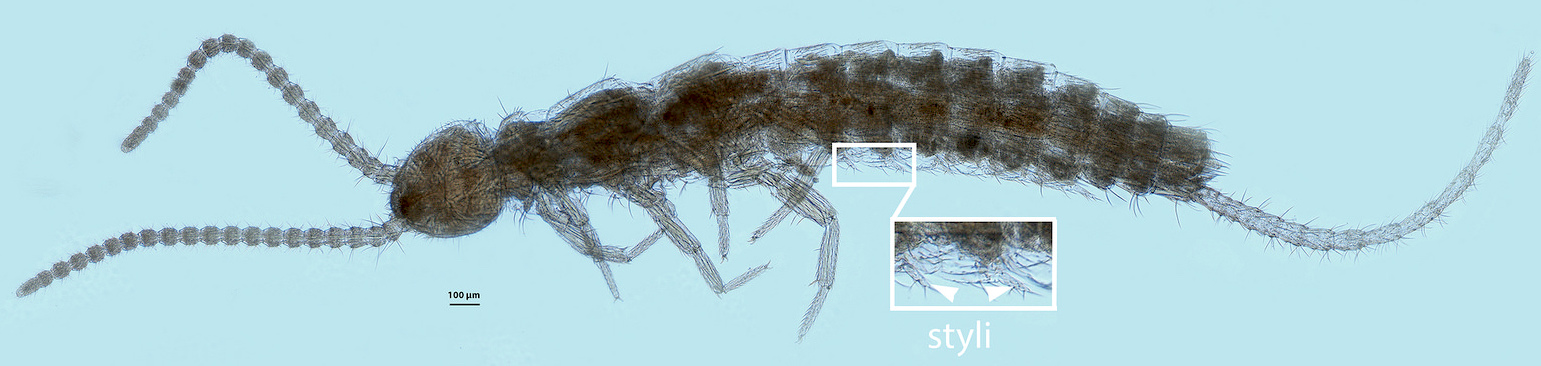
\includegraphics[width=0.9\textwidth]{campodeid1}
  \caption{Campodeidae habitus. Photo (CC BY 2.0) by Istv\'an Mik\'o \url{https://flic.kr/p/ykHVxt}}
  \label{fig:campodeidhab}
\end{figure}

\begin{figure}[ht!]
    \centering
    \begin{subfigure}[ht!]{0.45\textwidth}
        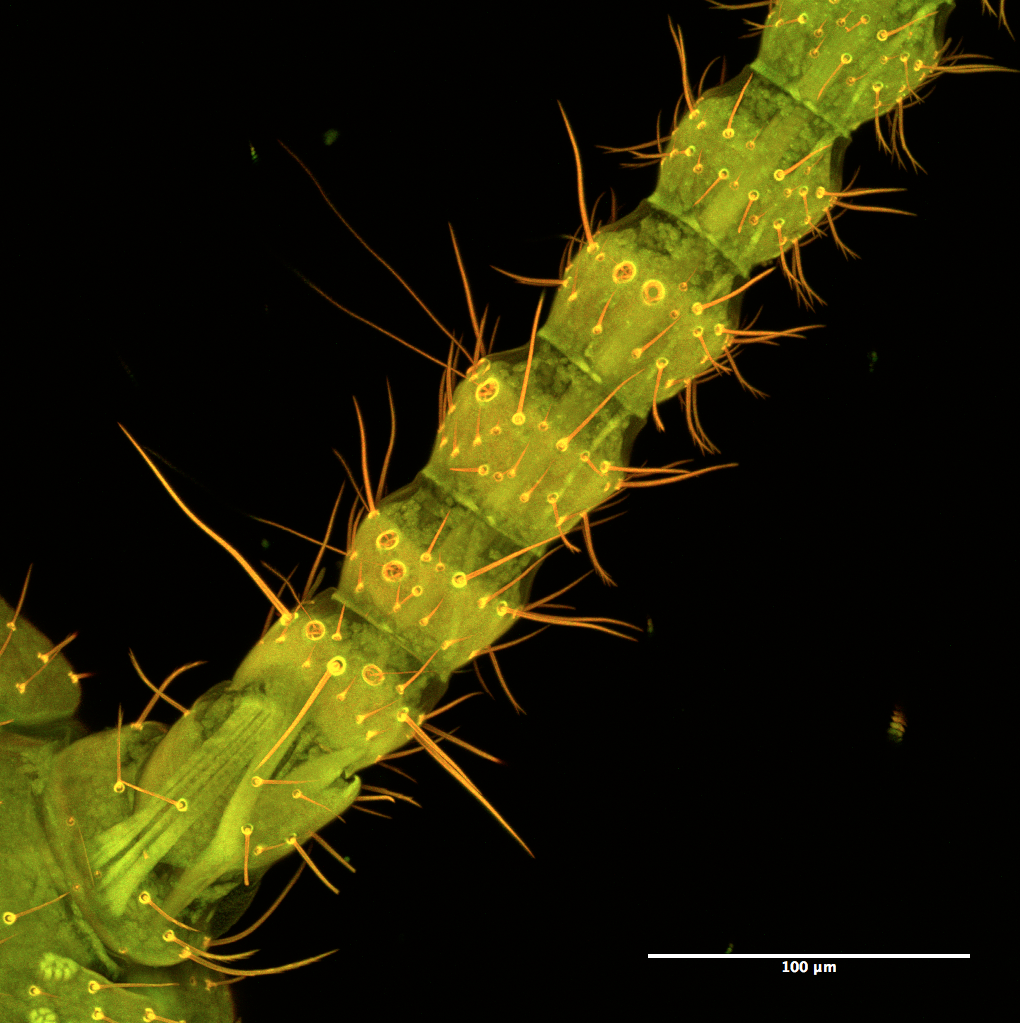
\includegraphics[width=\textwidth]{image11}
        \caption{External view}
        \label{fig:diplant1}
    \end{subfigure}
    ~ %add desired spacing between images, e. g. ~, \quad, \qquad, \hfill etc. 
      %(or a blank line to force the subfigure onto a new line)
    \begin{subfigure}[ht!]{0.45\textwidth}
        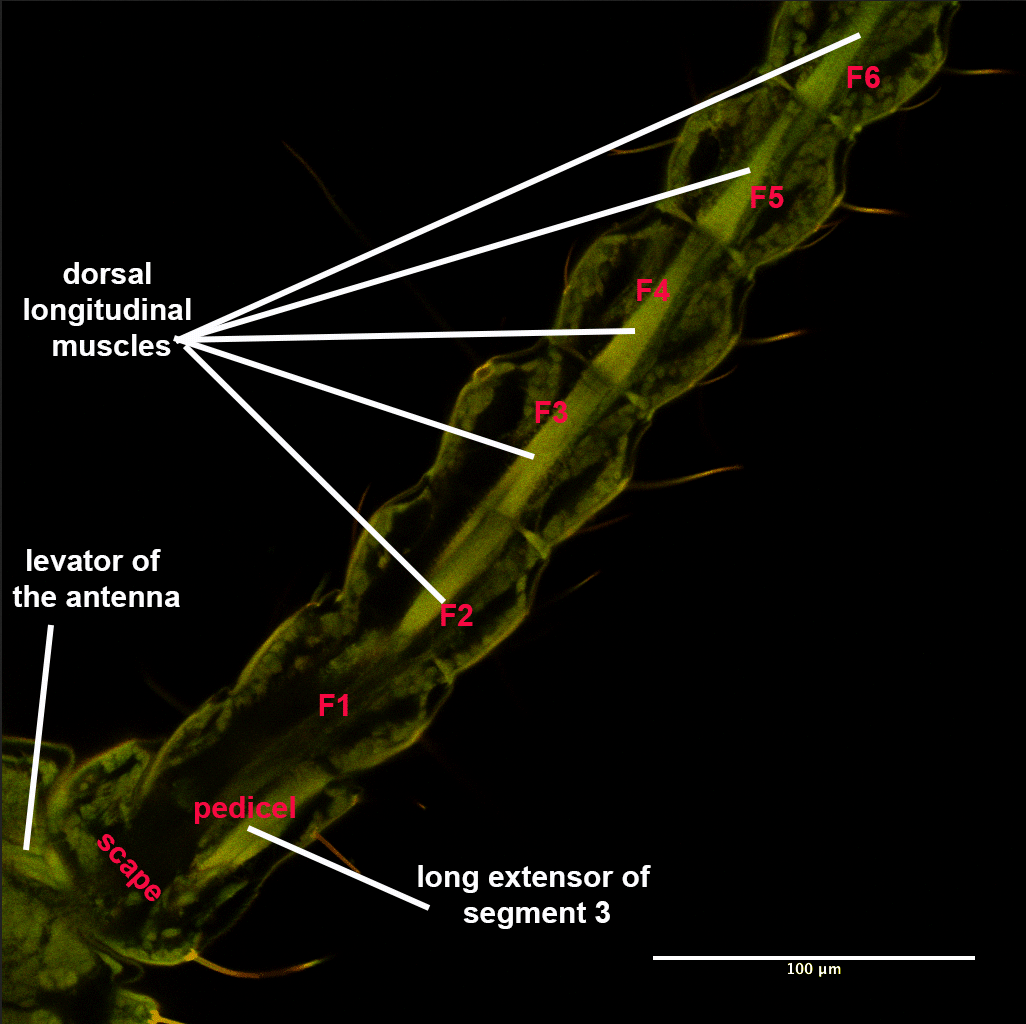
\includegraphics[width=\textwidth]{image26}
        \caption{Internal view, with muscles}
        \label{fig:diplant2}
    \end{subfigure}
    \caption{CLSM volume-rendered images, showing the antenna of Diplura. Photo (CC BY 2.0) by Istv\'an Mik\'o.}\label{fig:dipluraant}
\end{figure}

\begin{figure}[ht!]
    \centering
    \begin{subfigure}[ht!]{0.45\textwidth}
        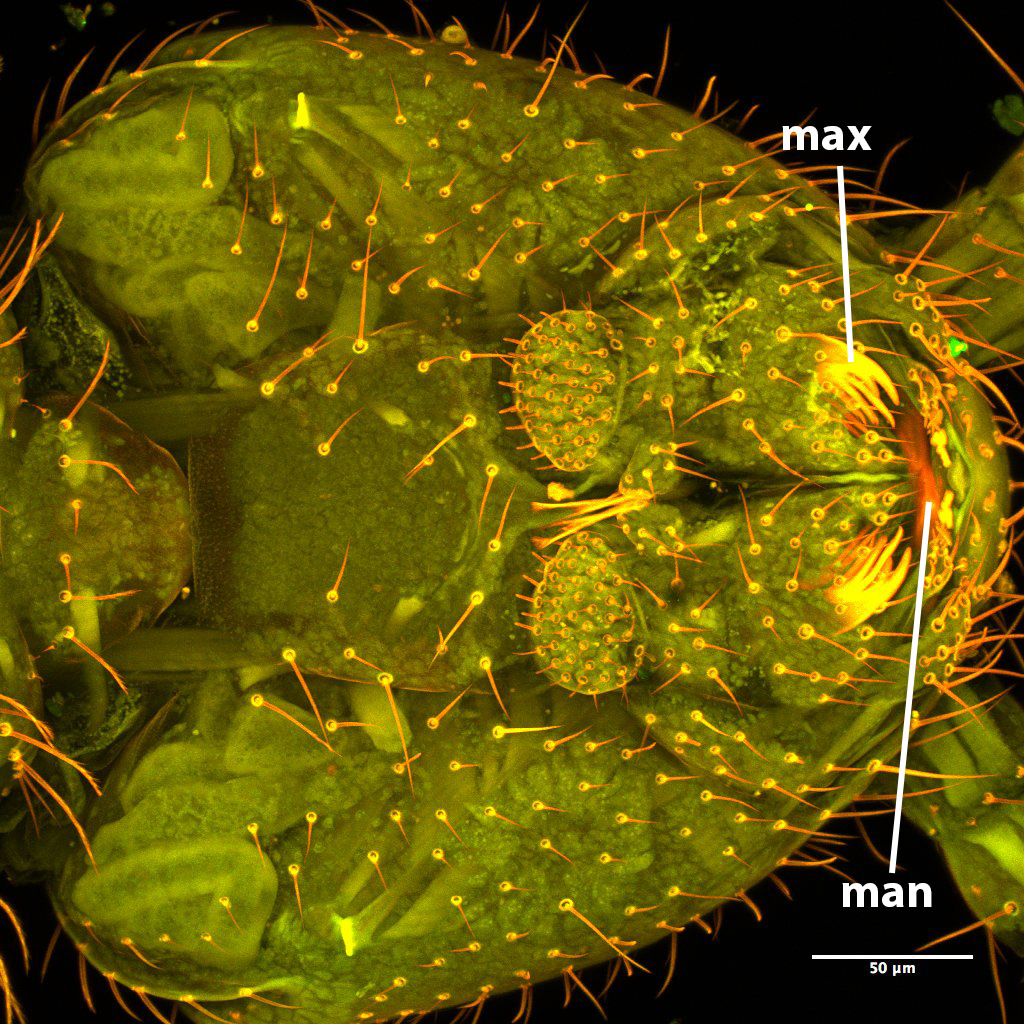
\includegraphics[width=\textwidth]{image33}
        \caption{Ventral view}
        \label{fig:dipheadvent}
    \end{subfigure}
    ~ %add desired spacing between images, e. g. ~, \quad, \qquad, \hfill etc. 
      %(or a blank line to force the subfigure onto a new line)
    \begin{subfigure}[ht!]{0.45\textwidth}
        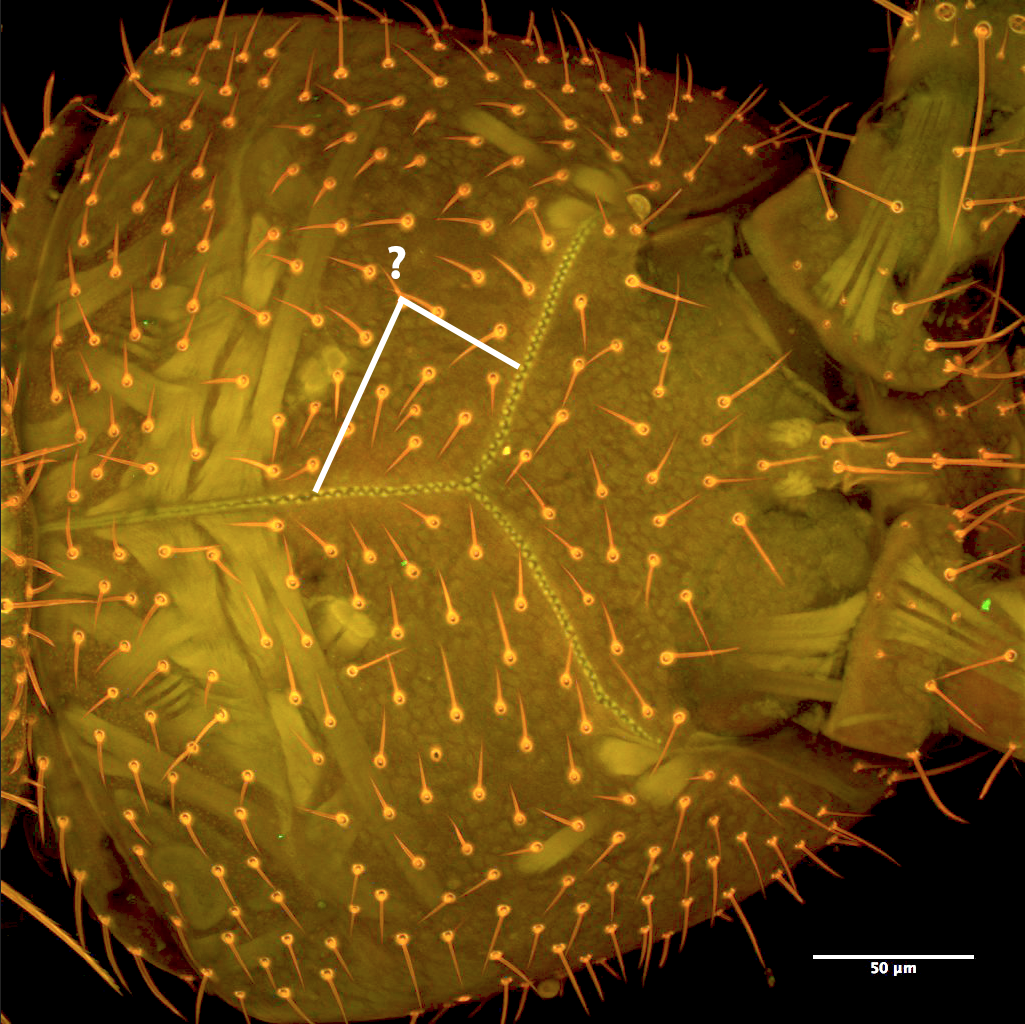
\includegraphics[width=\textwidth]{image04}
        \caption{Dorsal view, revealing suture}
        \label{fig:dipheaddors}
    \end{subfigure}
    \caption{CLSM volume-rendered images, showing the head of Diplura. Photo (CC BY 2.0) by Istv\'an Mik\'o}\label{fig:diplurahead}
\end{figure}

\section{Collembola (springtails)}
\begin{itemize}
\item compound eyes present
\item \textit{mandibles with molar area}
\item antennae usually $\leq$4 segments
\item tibia fused with tarsus (tibiotarsus)
\item abdomen with $\leq$6 segments: 1st segment with ventral tube (collophore), 3rd abdominal segment modified ventrally (retinaculum) to receive furculum, 5th abdominal segment with forked structure (furculum), usually folded under abdomen
\item body length usually 1--3 mm
\end{itemize}

\subsection{Sminthuridae (globular springtails)}
\begin{itemize}
\item head hypognathous, anteroposteriorly flattened
\item antennae longer than head
\item prothorax indistinct dorsally, narrowly articulated with head
\item abdominal segments 2--4 fused dorsally
\end{itemize}

\begin{figure}[ht!]
  \centering
    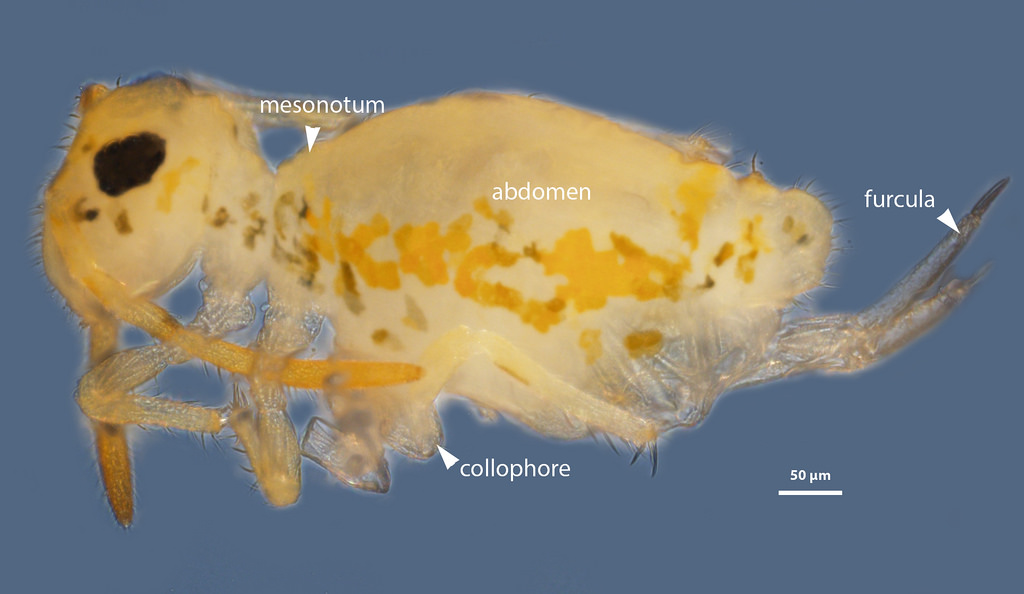
\includegraphics[width=0.8\textwidth]{sminthBody}
  \caption{Sminthuridae habitus. Photo (CC BY 2.0) by Istv\'an Mik\'o \url{https://flic.kr/p/xFw3ua)}}
  \label{fig:sminthhab}
\end{figure}

\subsection{Hypogastruridae (snowfleas, in part)}
\begin{itemize}
\item head prognathous, not anteroposteriorly flattened
\item antennae usually shorter than head
\item prothorax distinct dorsally, broadly articulated with head
\item abdominal segments 2--4 not fused
\end{itemize}

\begin{figure}[ht!]
  \centering
    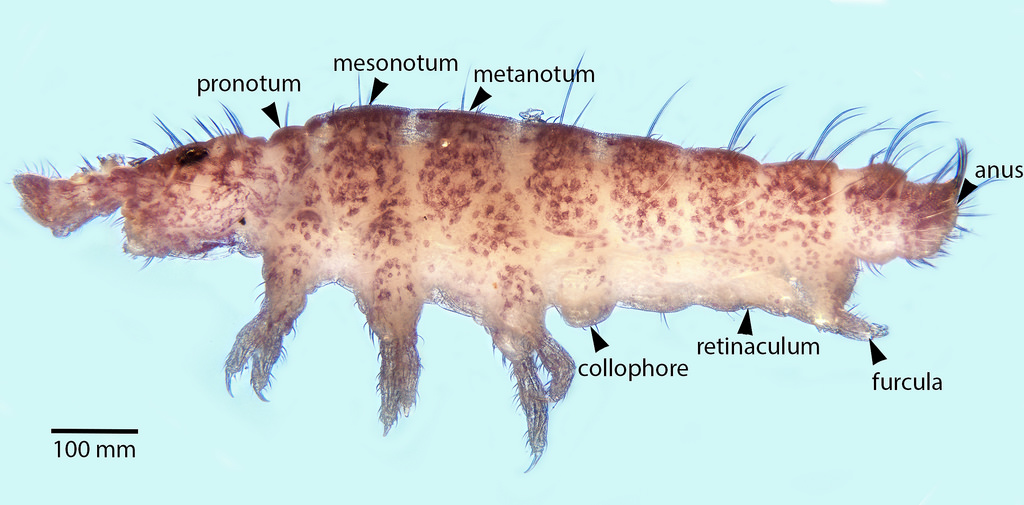
\includegraphics[width=0.8\textwidth]{hypogastrurid1}
  \caption{Hypogastruridae habitus. Photo (CC BY 2.0) by Istv\'an Mik\'o \url{https://flic.kr/p/ykEeQC}}
  \label{fig:hypogasthab}
\end{figure}

\subsection{Entomobryidae}
\begin{itemize}
\item head hypognathous to prognathous, not anteroposteriorly flattened
\item antennae longer than head
\item prothorax indistinct dorsally, narrowly articulated with head
\item abdominal segments 2--4 not fused
\end{itemize}

\begin{figure}[ht!]
  \centering
    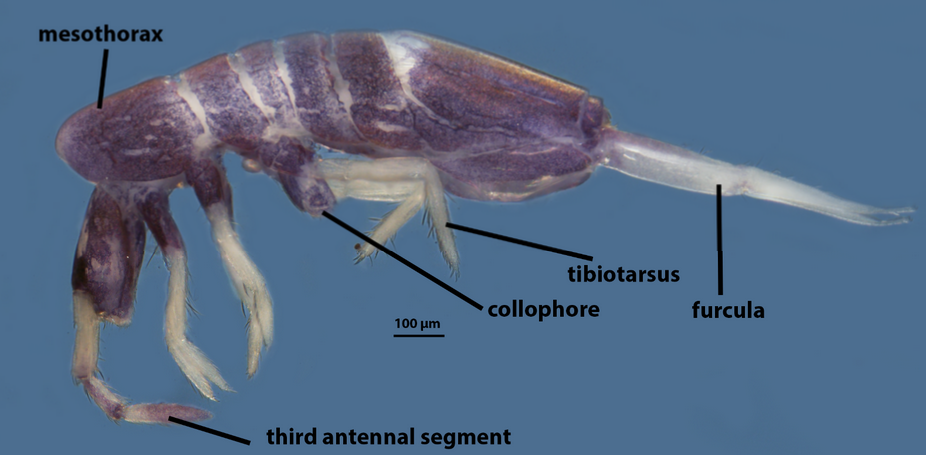
\includegraphics[width=0.8\textwidth]{entomobryid}
  \caption{Entomobryidae habitus. Photo (CC BY 2.0) by Istv\'an Mik\'o.}
  \label{fig:entomobry}
\end{figure}

\subsection{Tomoceridae}
\begin{itemize}
\item head hypognathous to prognathous, not anteroposteriorly flattened
\item antennae usually longer than head, apparently 3-segmented; apical segment longer than other 2 segments
\item prothorax indistinct dorsally, narrowly articulated with head
\item abdominal segments 2--4 not fused
\item often covered in metallic scales
\end{itemize}

\begin{figure}[ht!]
  \centering
    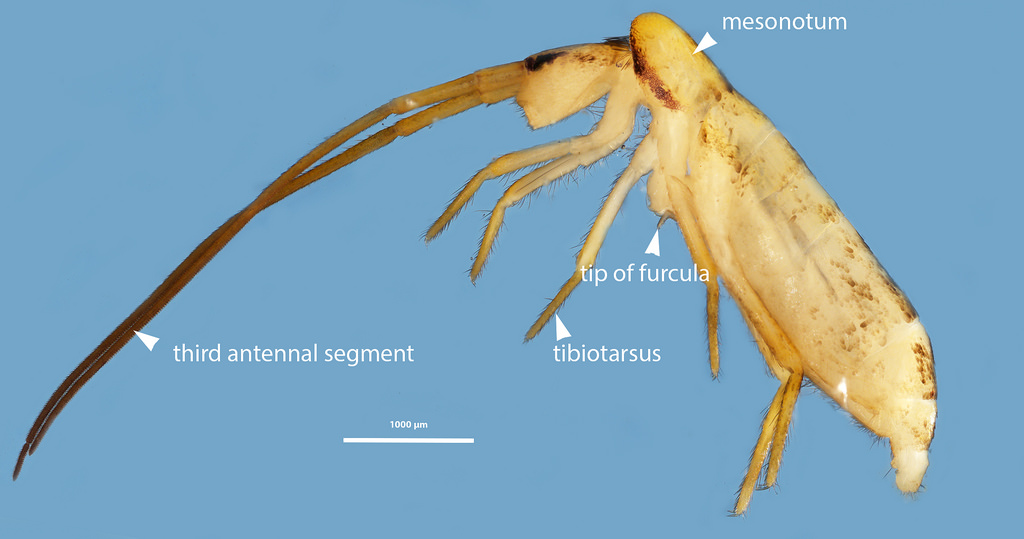
\includegraphics[width=0.8\textwidth]{tomo2}
  \caption{Tomoceridae habitus. Photo (CC BY 2.0) by Istv\'an Mik\'o https://flic.kr/p/yCnGYz}
  \label{fig:tomocer}
\end{figure}

\noindent{}Lines similar to the one marked on Figure \ref{fig:dipheaddors} occur on the epithelium of adult Entognatha. These structures are similar to human cranial sutures. What is their function? Winged insect adults do not have these lines, or at least they don't function in the same way. Why not?\vspace{3cm}

\section*{Insecta}
The remaining arthropods we will examine in lab are true insects. In addition to many internal characters we won't examine (\textit{e.g.}, Johnston's organ) insects can be recognized by the following character states:
\begin{itemize}
\item antennae 3-segmented (\textit{i.e.}, segments with intrinsic musculature), with apical segment (flagellum) usually subdivided
\item mouthparts not usually enveloped by cuticular evagination (\textit{i.e.}, insects are \textit{ectognathous})
\item ovipositor present
\end{itemize}

\section{Archaeognatha (Microcoryphia, bristletails)}
\begin{itemize}
\item compound eyes well-developed, adjacent dorsally
\item maxillary palps longer than legs, subdivided into 7 annuli
\item labial palps subdivided into 3 annuli
\item meso- and metacoxa with styli present
\item styli present on abdominal segments 2--9
\item abdomen with 3 scaly appendages present apically (2 cerci, 1 terminal appendage)
\item body ``humpbacked'', scaly
\item paired eversible vesicles usually present on abdominal segments 1--7
\end{itemize}

\begin{figure}[ht!]
  \centering
    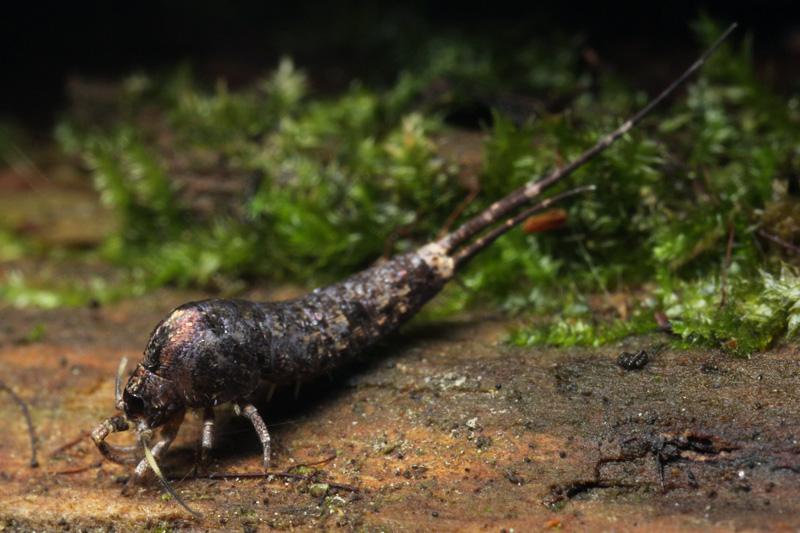
\includegraphics[width=0.8\textwidth]{image01}
  \caption{Archaeognathan habitus. Photo (CC BY-NC-SA 2.0) by Kim Fleming \url{https://flic.kr/p/5pYjac}}
  \label{fig:archhabit}
\end{figure}

\begin{figure}[ht!]
  \centering
    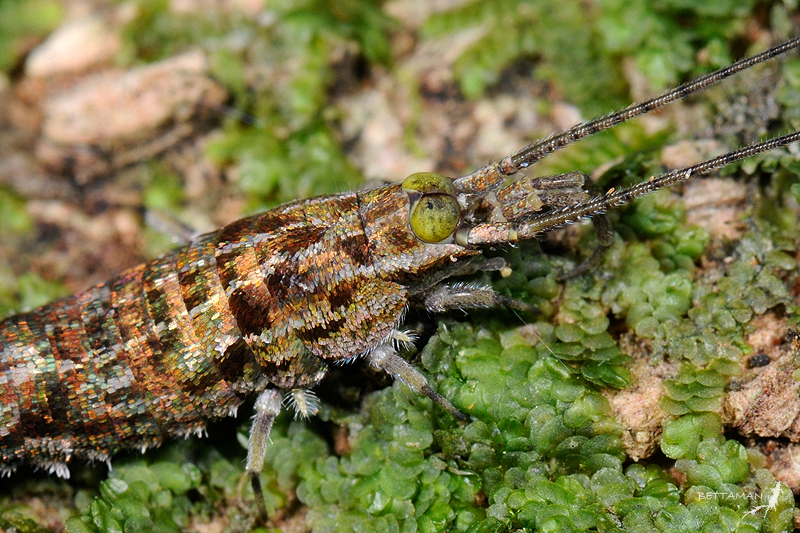
\includegraphics[width=0.7\textwidth]{image34}
  \caption{Archaeognathan head and thorax. Photo (CC BY-NC-SA 2.0) by Shipher Wu \url{https://flic.kr/p/62T1m3}}
  \label{fig:archhead}
\end{figure}

\noindent{}Have you seen these insects move? Why do they have a ``humpbacked'' habitus? Can you find and draw the styli? What might these be remnants of?\vspace{4cm}

\section{Zygentoma (Thysanura, in part; silverfish, firebrats)}

\begin{itemize}
\item compound eyes small, widely separated
\item maxillary palps shorter than legs, subdivided into 6 annuli
\item labial palps subdivided into 4 annuli
\item styli on meso- and metacoxa absent, usually present on abdominal segments 2--9 
\item abdomen with 3 bare appendages present apically (2 cerci, 1 terminal appendage)
\item body dorsoventrally flattened, scaly
\item paired eversible vesicles usually present on abdominal segments 1--7
\end{itemize}

\begin{figure}[ht!]
  \centering
    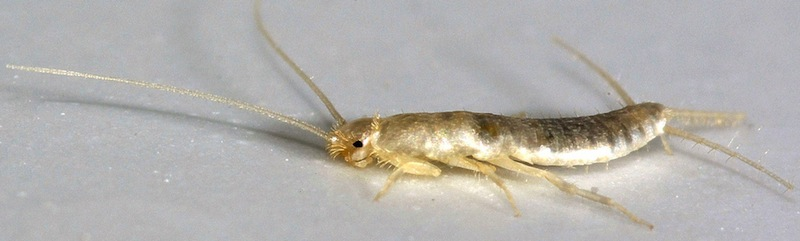
\includegraphics[width=0.8\textwidth]{image22}
  \caption{Zygentoman habitus. Photo (CC BY-SA 2.0) by Jean-Rapha\"el Guillaumin \url{https://flic.kr/p/4Cavhu}}
  \label{fig:zygenhabit}
\end{figure}

\begin{figure}[ht!]
  \centering
    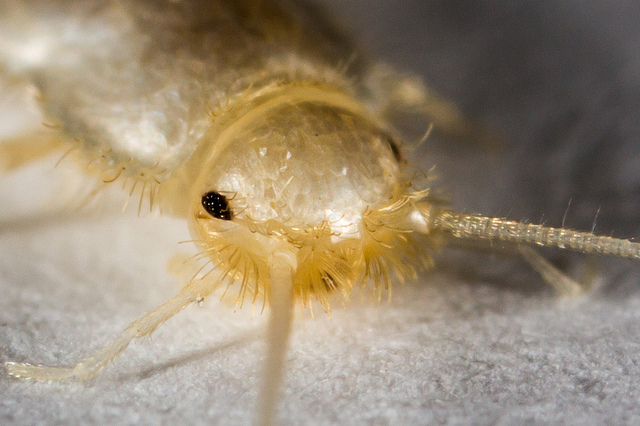
\includegraphics[width=0.8\textwidth]{image12}
  \caption{Zygentoman head. Photo (CC BY-SA 2.0) by Jean-Rapha\"el Guillaumin \url{https://flic.kr/p/czicq1}}
  \label{fig:zygenhead}
\end{figure}

\section*{Acknowledgments}
Andrew R. Deans and Istv\'an Mik\'o wrote the text. Many of the illustrations were generously made available by the Biodiversity Heritage Library (\url{http://biodiversitylibrary.org}) and the photographers at Flickr (\url{http://flickr.com}).
\FloatBarrier
% adding bibliography here
\bibliographystyle{apalike}
\bibliography{bib}
\end{document}
